\section{Evaluation}
\label{sec:semantic-eval}

% \subsection{Entry/Exit Comparison with Ground Truth}

\subsection{Tracking Accuracy with Scene Learning Filter}

The extracted movements and entry/exit locations are hard to evaluate quantitatively, due to a lack of both ground-truth and accepted difference metrics.
Instead, we extend a vehicle tracker with initialization- and update filters based on movements and entry/exit locations extracted from the scene, as described in the previous section.

\begin{figure}
    \centering
     \begin{subfigure}{0.48\linewidth}
    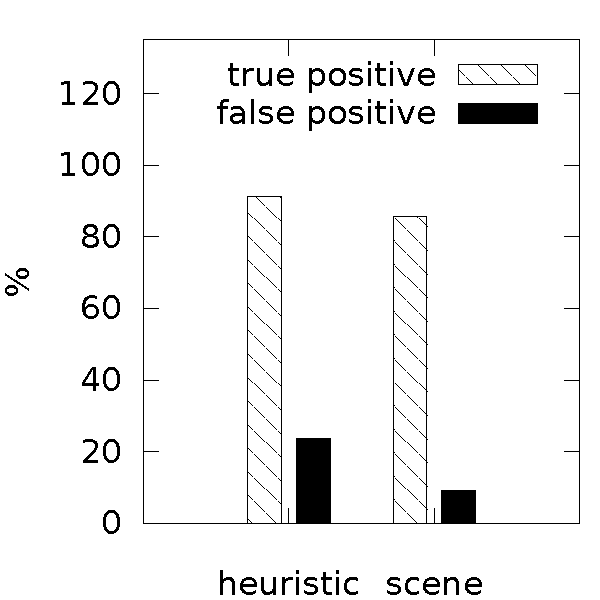
\includegraphics[width=\linewidth]{./img/semantic_tracker/exp/count_lowRes.pdf}
    \subcaption{Low resolution videos.}
    \end{subfigure}
    \begin{subfigure}{0.48\linewidth}
    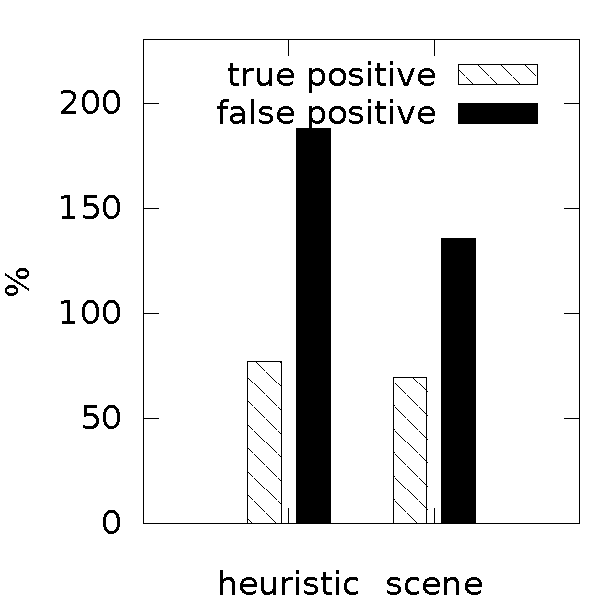
\includegraphics[width=\linewidth]{./img/semantic_tracker/exp/count_highRes.pdf}
            \subcaption{High resolution videos.}
    \end{subfigure}
    \caption{The number of true positive and false positve trackers. The black lines mark the ground truth, the striped and black bar are the true positive and false positive, separately.}
    \label{fig:semantic-eval-count}
\end{figure}

\ref{fig:semantic-eval-count} shows our main result. Here, we compare the tracker from \cite{yanziVehicleTracker}, labeled {\it heuristic}, against our version extended with a scene learning filter, labeled {\it scene}. 
Although the {\it heuristic} tracker relies on several manually tuned parameters, this is one of the few benchmarks that quantitatively evaluate tracking including initialization and termination, which is key for any realistic vehicle tracking application.

Here, true and false positives are based on matching tracked vehicles with ground truth trajectories.
We use the {\it overlap} of two rectangles, defined by the intersection over union for a rectangle box $\bm{r}$ and a ground truth $\bm{r}_0$,

$$\text{Overlap}(\bm{r}, \bm{r}_0) = \frac{A(\bm{r} \cap \bm{r}_0)}{A(\bm{r} \cup \bm{r}_0)},$$

averaged over the frames in which the ground truth trajectory or the tracking result occurs. 

As in \cite{yanziVehicleTracker}, we match each ground truth trajectory to the tracking result with the greatest overlap and use overlap $> 0.3$ to indicate a true positive. Any ground truth trajectories without a true positive match are considered false negatives, and any tracking result without a matched ground-truth trajectory with overlap > 0.3 is considered a false positive.
We find that our scene learning filter dramatically reduces false positives while keeping true positives essentially constant. 

A large number of false positives remain for the high-resolution videos. Due to the complex vehicle interactions in high the resolution video (see \ref{fig:entry-exit-full-3}), even with the semantic knowledge, the na\"ive Kalman Filter may easily lose track, resulting in an increased false positive count.

%We compare our scene-learning based tracker with the heuristic one, both with the setting that updated with background only and background along with detection, which we call BG and BG+DET. 
%According to the author, the dataset contains low-resolution videos with few occlusions and crowded high-resolution videos. We display their results separately for a better understanding of our method.

% \begin{itemize}
%         \item \textbf{Initialize}: A candidate rectangle $\bm{r}$ is not able to be initilialized with great overlap with any of the currently tracked objects $O_{\bm{r}}$, that is when $\text{IoU}(\bm{r}, O_{\bm{r}}) > 0.3$.
%         \item \textbf{Update}:An object $O_{\bm{r}}$ is updated with the rectangle $\bm{r}$ with the maximal $\text{IoU}(\bm{r}, O_{\bm{r}})$.
%         \item \textbf{Terminate}:Objects without update for 50 frames or out of image boundary are terminated.
%         \item \textbf{Validate}:Objects with lifetime longer than 50 frames and moves at last $\frac{1}{3}$ of the frame width is a good trajectory.
% \end{itemize}
% Here $\text{IoU}(\bm{r}_1, \bm{r}_2) = \frac{A(\bm{r}_1 \cap \bm{r}_2)}{A(\bm{r}_1 \cup \bm{r}_2)}$ is the widely used intersection over union metric. $\bm{r}_1 \cap \bm{r}_2$ and $\bm{r}_1 \cup \bm{r}_2$ representats the intersection and union separately, and $A(\cdot)$ simiply computes the area.

%With Eq. (\ref{eq:entry_score}), large number of candidate rectangles are filtered for initialization. In \ref{fig:filter-low} and \ref{fig:filter-high} shows the number of initialized and sucessfully tracked objects. For all the videos, semantic knowledge filters out up to $60\%$ more candidates than the heuristic tracker. 
%The successfully tracked object number proves the contribution of Eq. (\ref{eq:track_score}) and (\ref{eq:track_ext_score}) in filtering failed trackers. 
%% \begin{figure}
%%         \centering
%%          \begin{subfigure}{0.48\linewidth}
%%         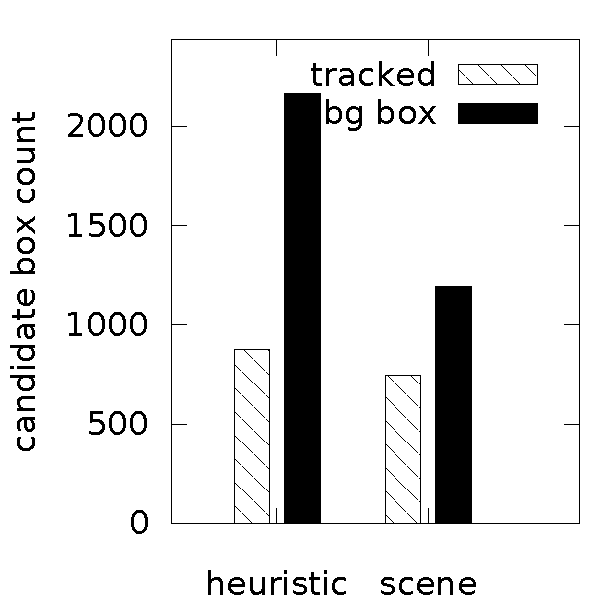
\includegraphics[width=\linewidth]{./img/exp/filter_BG_GPU_lowRes.pdf}
%%         \subcaption{Low resolution videos.}
%%         \end{subfigure}
%%         \begin{subfigure}{0.48\linewidth}
%%         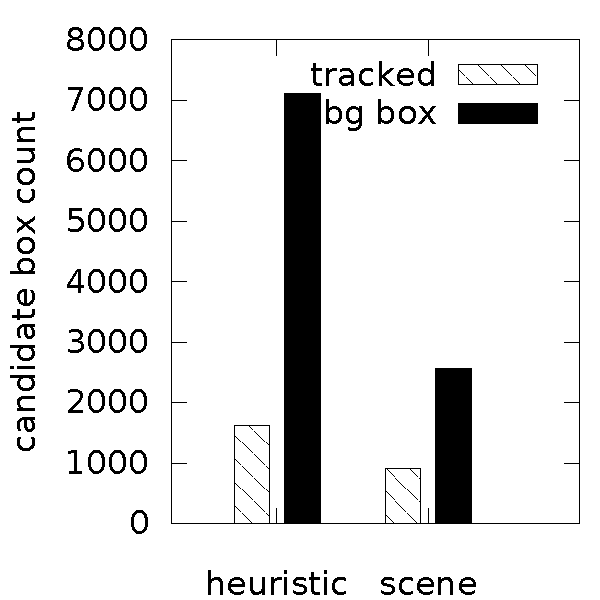
\includegraphics[width=\linewidth]{./img/exp/filter_BG_GPU_highRes.pdf}
%%         \subcaption{High resolution videos.}
%%         \end{subfigure}
%%         \caption{Initialization filtering for BG setting. The left group is heuristic tracker and the right is our tracker. The black bars are the number of objects initialized by background subtraction; the left striped bar is the sucessfully tracked objects number.}
%%         \label{fig:filter-low}
%% \end{figure}

%% \begin{figure}
%%         \centering
%%          \begin{subfigure}{0.48\linewidth}
%%         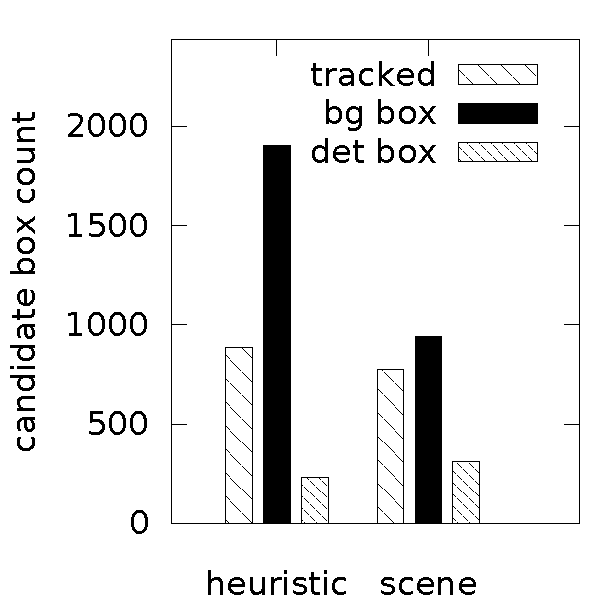
\includegraphics[width=\linewidth]{./img/exp/filter_BG+DET_lowRes.pdf}
%%         \subcaption{Low resolution videos.}
%%         \end{subfigure}
%%         \begin{subfigure}{0.48\linewidth}
%%         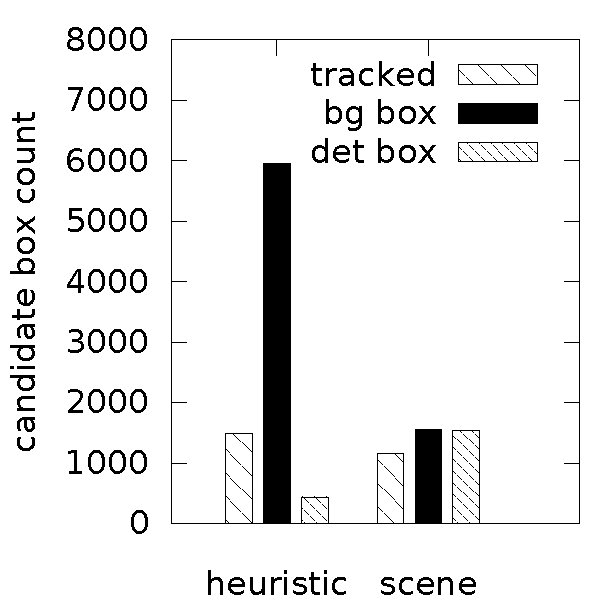
\includegraphics[width=\linewidth]{./img/exp/filter_BG+DET_highRes.pdf}
%%         \subcaption{High resolution videos.}
%%         \end{subfigure}
%%         \caption{Initialization filtering with BG+DET setting. The black and the right most bars in each group are the number of objects initialized by background subtraction and detector; the left striped bar is the sucessfully tracked objects number.}
%%         \label{fig:filter-high}
%% \end{figure}
%% The above figures show the semantic knowledge helps with eliminating noisy initializations and identifying tracking failure. 
%% Here we directly proves its improvement in tracking.
%% Ideally, a good tracker has true positives close to the ground truth, and false positives as few as possible.
%% \ref{fig:match} visualize the true positves and false positives of each tracker. 
%% Since there is no modification on the tracker self, it is reasonable that we don't have a significant change in true positives.
%% The scene knowledge integrated tracker maintains a roughly the same number of true positive, while dramatically reduces the false positive. 


%\subsection{Tracking accuracy}

\begin{figure}
    \centering
     \centering
     \begin{subfigure}{0.48\linewidth}
    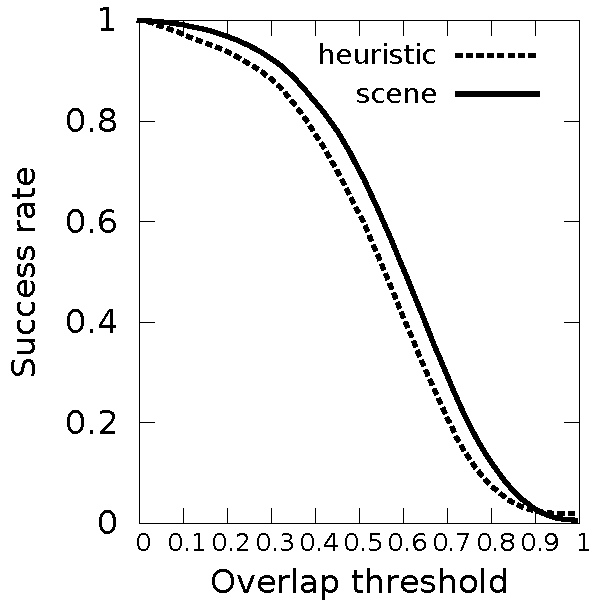
\includegraphics[width=\linewidth]{./img/semantic_tracker/exp/success_lowRes.pdf}
    \subcaption{Low resolution videos.}
    \end{subfigure}
    \begin{subfigure}{0.48\linewidth}
    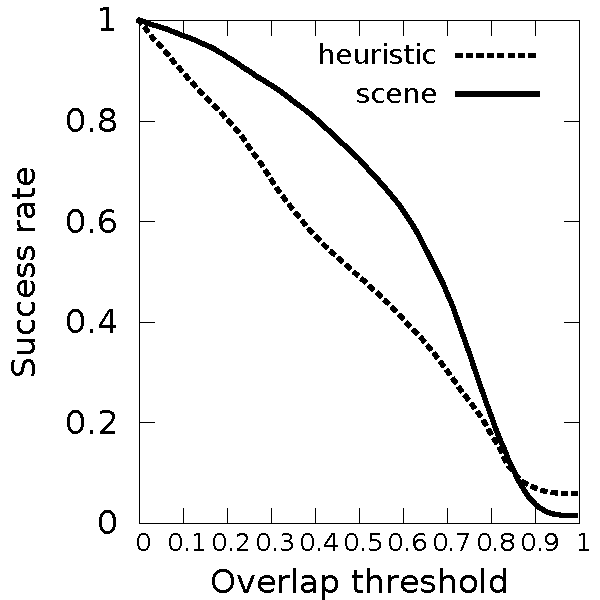
\includegraphics[width=\linewidth]{./img/semantic_tracker/exp/success_highRes.pdf}
            \subcaption{High resolution videos.}
    \end{subfigure}
    \caption{Success rate plot.}
    \label{fig:semantic-eval-success}
\end{figure}

\ref{fig:semantic-eval-success} shows the success plot of the two trackers for both simple and complex videos.
Here, the {\it success rate} is defined as the fraction ground-truth trajectories that have a minimum overlap with its matched tracking output.
Thus, the success rate measures how closely the matched trajectories actually match the ground truth.
The larger area under the curves is, the better the tracking is.
We see significant improvement in tracking accuracy with the help of scene learning, especially on the more complex videos.

%Without modification on the tracker, the improvement should come from a better initialization, which is consistent with the conclusion in \cite{yanziVehicleTracker}: for objects enters from the image boundary or coming from a tiny size, delaying the initialization could help improve the tracking performance.

In conclusion, we find that filtering tracker initialization and update using scene learning can significantly improve tracker performance, both in terms of precision and accuracy.  

%Our filtering criteria follow this conclusion in two ways: first, with the definition of the last point, objects are initialized only when it completely enters the image. That is to say, the corresponding tracker has richer information than the those initialized partially seen.
%Second, the topic model filters some noisy optical flows with tiny magnitude. 
%Therefore, the extracted entry location will not expand to the noisy area with small movements. Under our entry criteria, tiny objects will not be initialized until passing through a more confident region.
%Further with the experiments on the state-of-the-art trackers in \cite{yanziVehicleTracker}, the author concludes that general purpose trackers could benefit from proper initialization. 
%We could further infer that our semantic learning integrated initialization and tracking framework could be potentially useful any trackers in real-world use. 


% \subsection{Analysis of Semantic Tracking}
% Compare the ratio of initialization with maximal ground truth area with our last paper result.
